\hypertarget{ShipMap_8cpp}{}\section{Ship\+Map.\+cpp File Reference}
\label{ShipMap_8cpp}\index{Ship\+Map.\+cpp@{Ship\+Map.\+cpp}}


\hyperlink{classCheddar}{Cheddar} AI \hyperlink{classShipMap}{Ship\+Map} for Battleships.  


{\ttfamily \#include \char`\"{}Ship\+Map.\+h\char`\"{}}\\*
Include dependency graph for Ship\+Map.\+cpp\+:\nopagebreak
\begin{figure}[H]
\begin{center}
\leavevmode
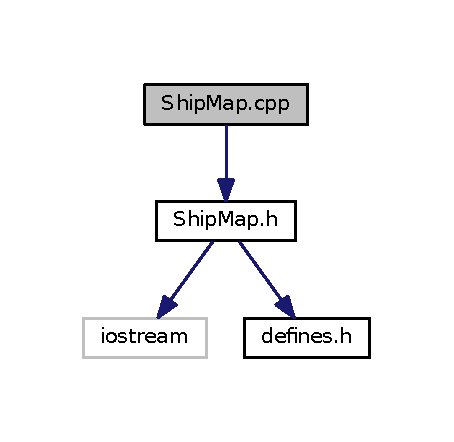
\includegraphics[width=218pt]{ShipMap_8cpp__incl}
\end{center}
\end{figure}


\subsection{Detailed Description}
\hyperlink{classCheddar}{Cheddar} AI \hyperlink{classShipMap}{Ship\+Map} for Battleships. 

\begin{DoxyAuthor}{Authors}
Jordan Wood, David Fletcher, Ryan Houck 
\end{DoxyAuthor}
\begin{DoxyDate}{Date}
April 14, 2018
\end{DoxyDate}
This class generates and maintains a map of where the enemy has shot. It can also give the index positions of the best place to put a ship of a given length, considering an opponent\textquotesingle{}s prior shooting pattern. 